%
%   Data description
%       - Importing data
%       - Data preprocessing
%       - Data cleaning
%   
\clearpage
\section{Data description}









\subsection{Overview of the dataset}

This dataset contains detailed specifications, release dates, and release prices of Intel CPUs. These specifications include some important attributes of a CPU,
and describes the performance (through \textit{Base frequency}), power consumption and heat (through \textit{Thermal design power}), and the technology trend (through
\textit{Number of cores} and \textit{Lithography}).

CPU (Central Processing Unit) is the most fundamental of a computer. CPU basically loads the instruction and execute it clock by clock, and produces return values.
Modern computers divides itself into many small processing units (called cores). During execution, it generates a lot of heat.

The dataset is retrieved from \href{https://www.kaggle.com/datasets/iliassekkaf/computerparts?select=Intel_CPUs.csv}{Computer Parts (CPUs and GPUs) Dataset (Kaggle)} 
by author Ilissek. Some notable attributes of this dataset are:

\begin{itemize}
    \item Vertical Segment (or Market segment) : describes which market a CPU is intended for. There are for markets segments: Mobile, Desktop, Embedded and Server. 
    \item Status : the current condition of the supply of CPU. They can be: Announce (incoming sales), Launched (currently active, fully supported), End of life (stop manufacturing, still supported) and
    End of interactive support (out of the support cycle).
    \item Launch date : the quarter-year date of which the CPU was available on the market.
    \item Lithography : the chip printing technique that was used to manufacture the CPU. Roughly speaking, as technology advances forward, this technique is getting smaller and smaller.
    \item Recommended Customer Price : the price recommended by Intel for retailers selling the CPU.
    \item Number of Cores : number of processing units on one CPU. More core does not mean better CPU. However, it helps utilizing parallel computing (multiple programs running at the same time).
    \item Base frequency : expected operating clock rate of a CPU. Larger frequency mean faster clock rate and therefore better performance.
    \item Thermal design power : theoretical heat and power consumption ceiling, the amount of heat needed to be cooled for normal operation of the CPU.
    \item Temperature (T) : the maximum temperature allowed on the CPU, before it could be damaged.
\end{itemize}










\subsection{Importing and Preprocessing}

\begin{code}{R}
pacman::p_load(
    rio,     # for dealing with basic import export
    ggplot2, # for dealing with plot formats
    zoo      # for dealing with year quarter formats
)

data <- import("./cpu-raw.csv") # rio::import

data <- data[, c("Vertical_Segment","Status","Launch_Date",
                 "Lithography","Recommended_Customer_Price",
                 "nb_of_Cores","Processor_Base_Frequency",
                 "TDP","T")] 
\end{code}

The primary packages used in this process are:

\begin{itemize}
    \item \verb|rio| : for intuitive I/O code.
    With this package, import and export dataset is easier and safer. It could 
    also handle multiple file formats, so that we do not have to
    change the command each time we change the file format.

    \item \verb|zoo| : for year-quarter format.
    In our data, the \verb|Launch date| is in non-standard format, and difficult to be operated on. This package helps to transform
    into standard year-quarter format, and provides useful operations, such as plotting and taking difference on these formats.

    \item \verb|ggplot2| : is a famous plotting package for R language.
\end{itemize}

The rest of the code is just choosing the attributes that are useful for our purpose.

The original labels are very long and descriptive, we might not want that such level of details during coding. Therefore, the labels are suppressed
into small, compact abbreviations. Then, we export the code to \verb|cpu-clean.csv|.

\begin{code}{R}
names(data) <- c("market", "status", "ldate", "litho", 
    "rprice", "ncore", "bfreq", "tdp", 
    "temp")

export("./cpu-clean.csv")
\end{code}









\subsection{Data cleaning}
\label{subsection:data_cleaning}

After choosing the approriate attributes, we now have the subset of the original raw dataset. 
However, since the values vary in types (such as string, non-standard year-quarter format and numeric-string),
we might want transform them into reproducible types, so that the analysis later on is easier, homogeneous and accurate.

Note that this cleaning process \textbf{does not} remove the \mintinline{R}{NA} values, unless necessary. The reason is that, 
in one instance, there might be important values that should not be eliminated. Under different scopes of study, we can not treat 
instances with \mintinline{R}{NA} as an invalid datum for all scopes. In later sections, when we focus on a specific pattern of the data, only by then
that the data will have a tailored \mintinline{R}{NA} cleaning, and we will not, by chance, loose any important instance.

This process took \verb|/rcode/cpu-short.csv| from the importing procedure above as an input, and produce \verb|/rcode/cpu-clean.csv| as
an output.

\begin{figure}[H]
    \centering
    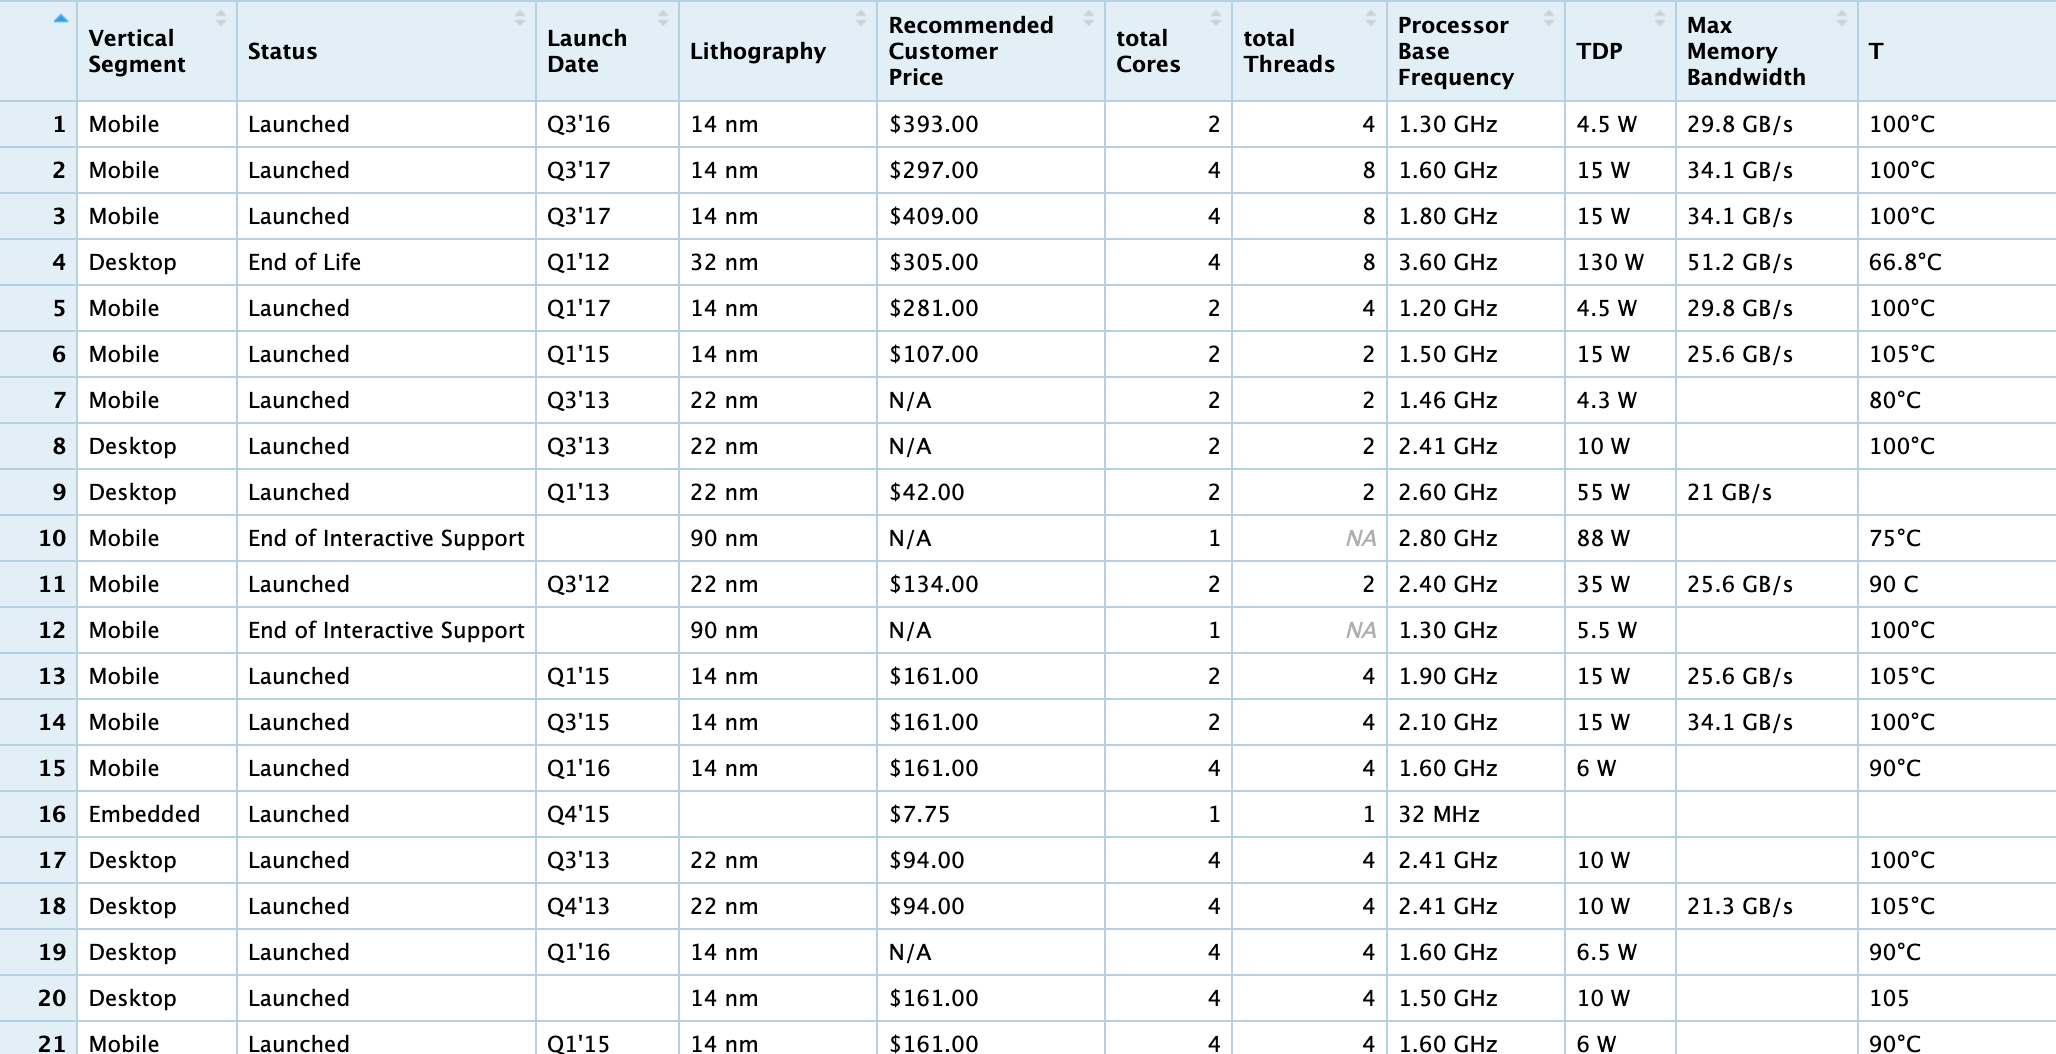
\includegraphics[max width=0.9\linewidth]{./graphics/short_data.png}
    \caption{Data before cleaning.}
\end{figure}

\verb|market| and \verb|status| are left unchanged, since the values are straightforward. The remaining attributes (columns) are processed as followed:

\subsubsection*{Launch dates (ldate)}

\begin{code}{R}
data[,"ldate"] <- (
    as.yearqtr(data[,"ldate"], format = "Q%q'%y")
)
\end{code}

Our goal is to transform raw, non-standard year-quarter into \verb|zoo|'s standards. 
The function \mintinline{R}{as.yearqtr} takes a column and a format string as parameters. The format string is represented 
as: \mintinline{R}{"Q%q'%y"}, in which two flags \mintinline{R}{"%q"}, \mintinline{R}{"%y"} stands for quarter and year, respectively.
The format string hints the function to know the positions of quarter and year in our raw string.

\subsubsection*{Lithography (litho)}

\begin{code}{R}
data[,"litho"] <- as.numeric(
    gsub(" nm", "", data[,"litho"])
)
\end{code}

Our goal is to cut out \verb|"nm"|, since every entry is recorded in nanometers anyway. In this code, \verb|gsub| substitutes 
the pattern \verb|" nm"| to \verb|""|. Notice that the pattern are regular expressions, and would be used intensively during 
this cleaning process (See \textbf{Section \nameref{section:appendix:regex}} for more details).

\subsubsection*{Recommended Customer Price (rprice)}

\begin{code}{R}
data[,"rprice"] <- gsub(
    "(^\\$(\\d)+.(\\d)+ - )", 
    "", 
    data[,"rprice"]
)

data$rprice <- ifelse(data$rprice == "N/A", NA, data$rprice)

data$rprice <- as.numeric(gsub('\\$|,', '', data$rprice))
\end{code}

Some \verb|rprice| values have ranges instead of sole numbers. We want to cut out uneccesary characters and only keep the largest price.
After that, we eliminate \verb|$| symbol from the string, as well as cast the string to numeric type.

\subsubsection*{Base frequency (bfreq)}

\begin{code}{R}
data[,"bfreq"] <- as.numeric(
    gsub("( GHz)|( MHz)", "", data[,"bfreq"])
)

data<- data[!is.na(data$bfreq), ]

data$bfreq[data$bfreq > 10] <- data$bfreq[data$bfreq > 10]*0.001
\end{code}

Our goal is to cut out \verb|"GHz"| and \verb|"MHz"| from the string, and convert all \verb|"MHz"| values into \verb|"GHz"|. Heuristically,
we observed that any value greater than 10 must be \verb|MHz|, so we can transform every value like that will be multiply by 0.001 to get 
the according \verb|MHz| value.

\subsubsection*{Thermal design power (TDP)}

\begin{code}{R}
data[,"tdp"] <- as.numeric(
    gsub(" W", "", data[,"tdp"])
)    
\end{code}

\subsubsection*{Temperature (temp)}

\begin{code}{R}
data[,"temp"] <- (gsub("[^0-9.\\-]+", ",", data[,"temp"]))
for (i in seq_along(data[["temp"]])) {
    temp_values <- strsplit(data[i, "temp"], ",") 
    temp_values <- unlist(lapply(temp_values, as.numeric))
    max_value <- max(temp_values, na.rm = TRUE)
    if (is.infinite(max_value)) {
        max_value <- NA
    }
    data[i, "temp"] <- max_value
}

export(data, "cpu-clean.csv")
\end{code}

Our goal is to only match the numeric values, then, take the maximum among those. The approach to processing the complicated strings in \verb|temp| is described as follows:
\begin{itemize}
    \item First, we attempt to match every decimal numbers possible, including the irrelevant number. The rest are replaced with commas \verb|","|.
    The result of this process will create a string of numbers separated by commas. By doing this, the numbers are well isolated for our purpose.

    \item Second, we split these numbers and form a vector of them. This can be done through \mintinline{R}{strsplit} function. Notice that our numbers
    are still in string format.

    \item Third, we cast all these strings to numeric and push them into a vector of values using \mintinline{R}{unlist} and \mintinline{R}{lapply}
    
    \item Fourth, we find the maximum among all these values. Invalid numbers will automatically become \(-\infty\), and will be further treated as \mintinline{R}{NA}.
    
    \item Notice that, we must loop through each row of the list to accomplish the above procedure.
\end{itemize}

Finally, the program produces \verb|cpu-clean.csv| as a cleaned data, ready for further exploitation in the later sections.

\begin{figure}[H]
    \centering
    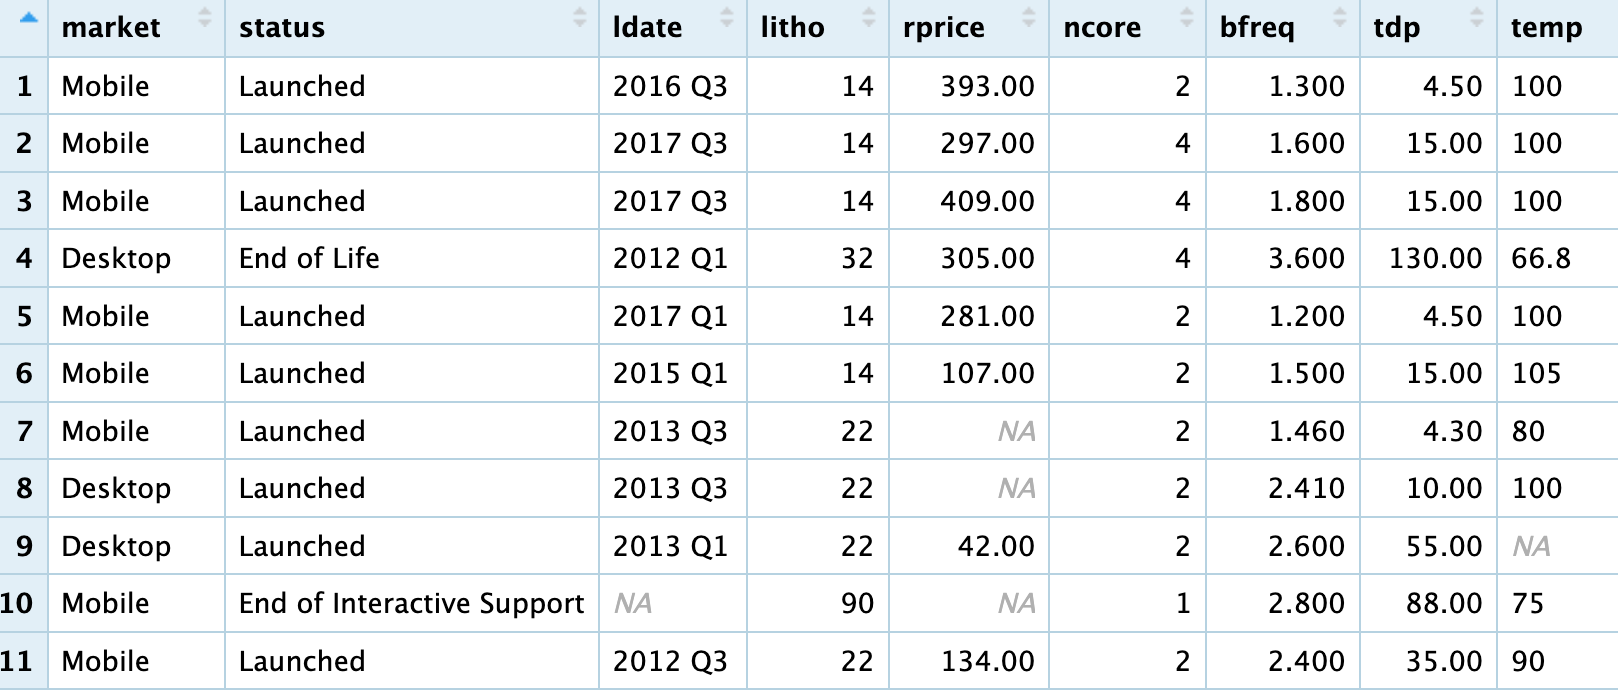
\includegraphics[max width=0.9\linewidth]{./graphics/cleaned_data.png}
    \caption{Data after cleaning.}
\end{figure}

% END OF DATA CLEANING